
\chapter{Virtualization}

\textbf{Virtualization} uses software to create an \textit{abstraction layer} over computer hardware that allows the hardware elements of a single computer - processors, memory, storage and more - to be divided into multiple virtual computers, commonly called virtual machines (VMs). Each VM runs its own operating system (OS) and behaves like an independent computer, even though it is running on just a portion of the actual underlying computer hardware. 
\begin{figure}[H]
    \centering
    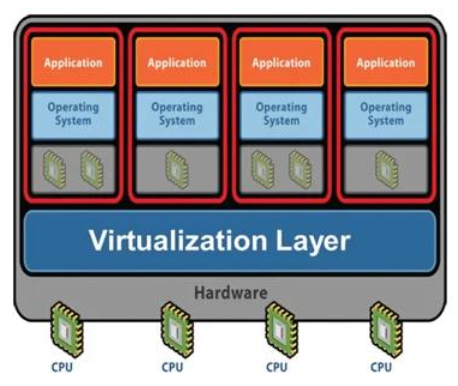
\includegraphics[width=0.5\textwidth]{assets/fig27.png}
    \caption{Virtualization}
\end{figure}

It is the ability to “simulate” a hardware platform, such as a server,
storage device or network resource, in software. All the functionality is separated
(abstracted) from the hardware and “simulated” as a “virtual instance” with the ability to
operate just like the hardware solution. A single hardware platform can be used to support
multiple virtual devices or machines, which are easy to spin up or down as needed.

\textbf{Virtual Machine} refers to a software simulation of a computer. It can run an OS and applications interacting with the virtualized abstracted resources, \textit{not with the physical resources} of the actual host computer.

\textbf{Hypervisor (or VM monitor)} refers to a software tool installed on the physical host system to provide the this software layer of abstraction that decouples the OS from the physical bare-metal. It allows to split a computer in different separate environments, the VMs, distributing them the computer resources. 

Components:

\begin{itemize}
    \item \textbf{Host OS}: the OS running on the physical machine.
    \item \textbf{Hypervisor}: the software layer that abstracts the hardware and creates the VMs.
    \item \textbf{Guest OS}: the OS running on the VM.
\end{itemize}

\begin{figure}[H]
    \centering
    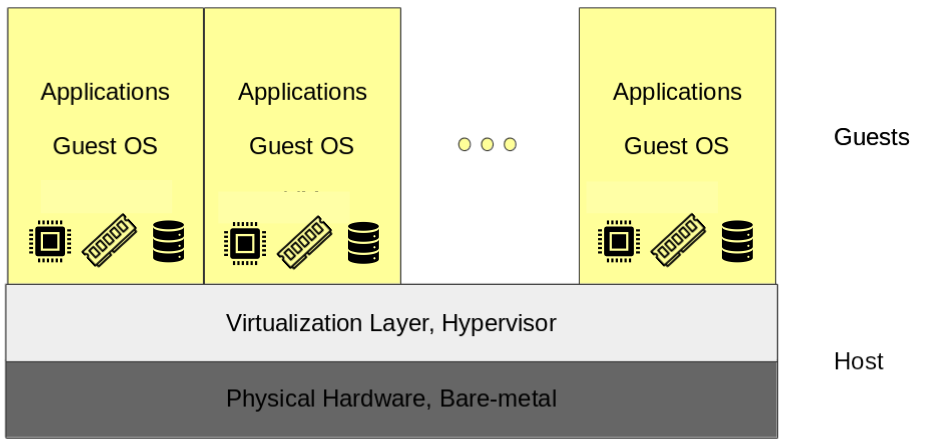
\includegraphics[width=0.5\textwidth]{assets/fig28.png}
    \caption{Virtualization components}
\end{figure}

\section{Virtual Machines}

A Virtual Machine is a virtual computing system. It has tighly \textbf{isolated} software with an OS and applications inside. Each VM in a host is \textbf{independent}. 

In a single physical server can be put multiple VMs enabling the run of multiple OSes and Applications (\textit{partition/multi-tenancy}).

Features:
\begin{itemize}
    \item \textbf{Consolidation}: multiple VMs on a single physical server.
    \item \textbf{Isolation}: VMs are independent.
    \item \textbf{Encapsulation}: VMs are portable.
    \item \textbf{Hardware Independence}: VMs are not tied to the physical hardware.
    \item \textbf{Security}: VMs are isolated from each other.
\end{itemize}

\section{Virtualization models}

\begin{figure}[H]
    \centering
    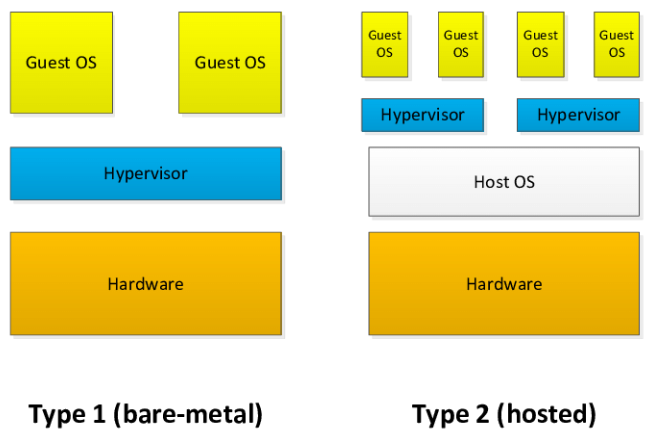
\includegraphics[width=0.5\textwidth]{assets/fig29.png}
    \caption{Virtualization models}
\end{figure}

\begin{enumerate}
    \item \textbf{Type 1 Hypervisor}: it runs directly on the host's hardware to control the hardware and to manage guest operating systems. It is also called \textit{bare metal hypervisor}. It is the most efficient because it has direct access to the hardware. Examples: VMware ESXi, Microsoft Hyper-V, Citrix XenServer, Oracle VM Server for SPARC.
    \item \textbf{Type 2 Hypervisor}: it runs on a conventional operating system just as other computer programs do. It is also called \textit{hosted hypervisor}. It is easier to set up and use, but it is less efficient because it must use the host OS to access the hardware. Examples: VMware Workstation, VMware Player, Oracle VirtualBox, Parallels Desktop for Mac.
\end{enumerate}

Another distinction can be made w.r.t. virtualization:
\begin{itemize}
    \item \textbf{Full virtualization}: the hypervisor provides complete hardware abstraction creating
    simulated hardware devices. The guest OS don’t know (or care) about the presence
    of a hypervisor and issue commands to what it thinks is actual hardware.
    \item \textbf{Paravirtualization}: the guest OS is aware of the hypervisor and interacts with it
    \item \textbf{Hardware-assisted virtualization}: the hypervisor uses hardware capabilities to
\end{itemize}

\begin{warningblock}[Hardware Protection Levels]
    Since computers run more than on software process, this will bring some issues. Protection rings are one of the key solutions for sharing resources and hardware.
    \begin{itemize}
        \item \textbf{Ring 0}: the most privileged level (kernel mode).
        \item \textbf{Ring 1-2-3}: less privileged levels (user mode).
    \end{itemize}
    The hypervisor runs in Ring 0, the guest OS runs in Ring 1-2-3.
\end{warningblock}

\section{Virtualizing components}

\subsection{CPU}

The hypervisor must manage the CPU resources. It must decide which VM gets CPU time and when. It must also manage the CPU instructions that are executed by the VMs.

Guest instructions are executed directly by the hardware as much as
possible: virtual machine monitor does not interfere with every single
instruction that is issued by the guest operating system, or its applications.
The non-privileged instructions will operate at hardware speeds.

\textbf{Privileged instructions}: Whenever a privileged instruction gets accessed,
then the processor causes a trap, and control is automatically switched to
the most privileged level, that is the hypervisor. At this point, the
hypervisor can determine whether the operation is to be an allowed or
not. Illegal operations will cause actions on the VM (as KILL), legal
operations the hypervisor should perform the necessary emulation so
that the guest operating system is under the impression that it does have
control over the hardware.

\subsection{Memory}

\textbf{Full virtualization}: the guest operating system continues to observe a
contiguous linear physical address space that starts from physical
address 0.
Three types of addresses:
\begin{itemize}
    \item \textbf{Virtual addresses}, these are the ones that are used by the applications in the guest
    \item \textbf{Physical addresses}, these are the ones that the guest thinks are the addresses of the physical resources 
    \item \textbf{The machine addresses}, these are the actual machine addresses with the actual physical addresses on the underlying platform. 
\end{itemize}

\begin{figure}[H]
    \centering
    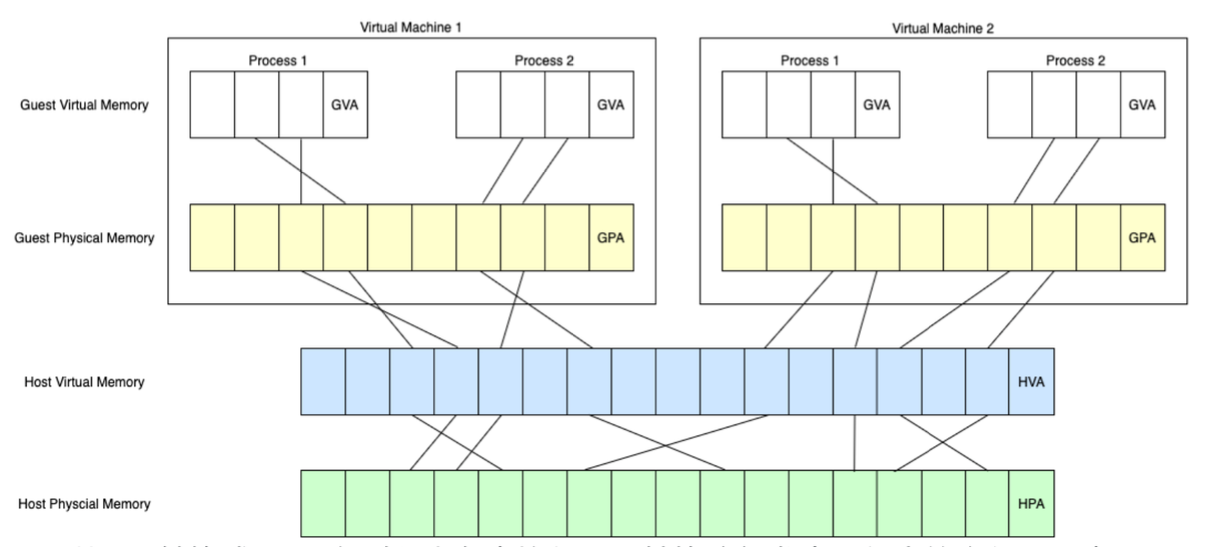
\includegraphics[width=0.8\textwidth]{assets/fig30.png}
    \caption{Memory virtualization}
\end{figure}

Every single memory access goes through two separate translation, the first one
which will be done in software, and then the second one potentially can take
advantage of hardware.

Moreover, \textbf{Shadow Page Table} estabilishes a shortcut to directly manage the mapping from GVA to HPA. It works the same way virtual addresses is mapped to physical addresses. VMM must maintain consistence between the page tables.

\begin{figure}[H]
    \centering
    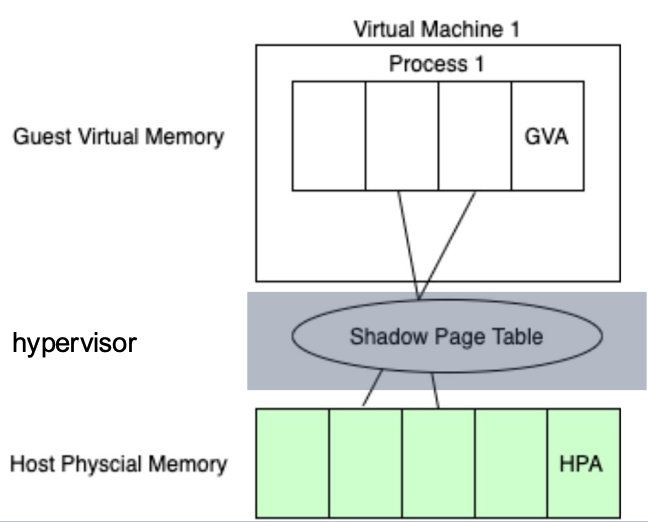
\includegraphics[width=0.5\textwidth]{assets/fig31.png}
    \caption{Shadow Page Table}
\end{figure}

\textbf{Paravirtualization} allows guest operating systems to be aware of their virtual environment 
and communicate directly with the hypervisor to manage memory. 
Instead of fully abstracting the underlying hardware, the guest OS uses an optimized 
interface to reduce the overhead of trapping into privileged operations. 
This approach decreases the complexity of mapping guest physical addresses to machine 
addresses by enabling the hypervisor and guest OS to collaborate on page table management 
and memory access, leading to more efficient performance overall.

\subsection{Network}

The hypervisor must manage the network resources. It must decide which VM gets network access and when. It must also manage the network packets that are sent and received by the VMs. Applications run on a virtual network as they
where running on a physical network.

\begin{itemize}
    \item \textbf{Flexibility}: VMs can be moved between physical servers without changing the network configuration.
    \item \textbf{Manageability}: VMs can be managed as a single entity.
    \item \textbf{Scalability}: VMs can be added or removed as needed.
    \item \textbf{Security}: VMs are isolated from each other.
    \item \textbf{Programmability}: VMs can be controlled by software.
    \item \textbf{Heterogeneity}: VMs can run different OSes and applications.
\end{itemize}

\begin{figure}[H]
    \centering
    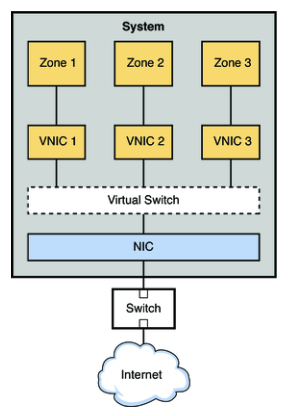
\includegraphics[width=0.5\textwidth]{assets/fig32.png}
    \caption{Network virtualization}
\end{figure}

\subsection{Disk}

The hypervisor must manage the disk resources. It must decide which VM gets disk access and when. It must also manage the disk blocks that are read and written by the VMs. Applications run on a virtual disk as they where running on a physical disk.
Virtual Disks are where guest operating systems are installed, making them the
equivalent of traditional hard disks. They are stored as files on the host system’s
physical disk.

\begin{itemize}
    \item \textbf{Flexibility}: VMs can be moved between physical servers without changing the disk configuration.
    \item \textbf{Manageability}: VMs can be managed as a single entity.
    \item \textbf{Scalability}: VMs can be added or removed as needed.
    \item \textbf{Security}: VMs are isolated from each other.
    \item \textbf{Programmability}: VMs can be controlled by software.
    \item \textbf{Heterogeneity}: VMs can run different OSes and applications.
\end{itemize}

\section{Emulation}

\textbf{Emulation} is the process of simulating hardware using software. It is used when the guest OS is not aware of the hypervisor. The hypervisor must emulate the hardware that the guest OS expects to see.

Emulation brings higher overhead but has its perks too. It is highly inexpensive, easy to access,
and helps us run the programs that have become obsolete in the available system. Anyone can access the emulation platforms remotely and is easier to use. It is an excellent
ability to have for embedded/OS development, without affecting the underlying OS.

